\subsection{Ca sử dụng tổng hợp lịch trình từ hội thoại}
\noindent Ca sử dụng này mô tả cách hệ thống tự động tổng hợp và đề xuất lịch trình dựa trên nội dung các tin nhắn trong một cuộc hội thoại nhóm. Hệ thống sử dụng AI để phân tích tin nhắn, nhận diện các hoạt động, địa điểm, thời gian và tạo ra một lịch trình có cấu trúc. Bảng~\ref{tab:uc_summarize_itinerary_spec} trình bày chi tiết đặc tả ca sử dụng, bao gồm luồng sự kiện chính, luồng thay thế, các điều kiện và yêu cầu liên quan. Các biểu đồ hoạt động, quan hệ (Bảng~\ref{tab:uc_summarize_itinerary_diagrams}) và tuần tự (Hình~\ref{fig:3-3-10-sequence-diagram}) minh họa rõ hơn về quy trình và tương tác hệ thống khi thực hiện tổng hợp lịch trình.
% \vspace{0.5cm} % Adjust spacing if needed

% Use longtable environment
% Need \usepackage{longtable} and \usepackage{calc} in preamble
\begin{longtable}{| p{4cm} | p{\dimexpr\linewidth-4cm-4\tabcolsep} |} % Adjust widths as needed
    \caption{Đặc tả ca sử dụng tổng hợp lịch trình từ hội thoại} % Caption inside longtable
    \label{tab:uc_summarize_itinerary_spec} \\ % Label after caption

    \hline
    \textbf{Mô tả} & Hệ thống sẽ tổng hợp lại lịch trình được đúc kết từ đoạn tin nhắn trong nhóm chat của người dùng. \\
    \hline
    \endfirsthead % Header for the first page

    % No \endhead content needed

    % No \endfoot content needed

    \hline % Footer for the last page
    \endlastfoot

    % --- Table Content ---
    \textbf{Luồng cơ bản} & 1. Người dùng bấm vào một cuộc hội thoại nhóm muốn tổng hợp. \newline
                           2. Hệ thống hiển thị thông tin cuộc hội thoại và các tin nhắn trong cuộc hội thoại đó. \newline
                           3. Người dùng chọn tùy chọn tổng hợp tin nhắn. \newline
                           4. Hệ thống lấy và hiển thị lịch trình tổng hợp của cuộc hội thoại (nếu có). \newline
                           5. Người dùng bấm ``Tổng hợp". \newline
                           6. Hệ thống sử dụng AI tổng hợp lịch trình trong cuộc hội thoại và hiển thị lịch trình tổng hợp. \\
    \hline
    \textbf{Luồng thay thế} & Hệ thống thông báo lỗi khi không có tin nhắn mới chưa được cập nhật hoặc khi quá trình tổng hợp AI gặp sự cố. \\
    \hline
    \textbf{Tiền điều kiện} & - Người dùng đang đăng nhập và phiên đăng nhập chưa kết thúc. \newline
                           - Người dùng đã có ít nhất một cuộc hội thoại nhóm. \\
    \hline
    \textbf{Hậu điều kiện} & - Hệ thống tổng hợp lịch trình sau đó lưu vào cơ sở dữ liệu và hiển thị cho người dùng. \newline
                           - Hệ thống đánh dấu các tin nhắn đã được tổng hợp. \newline
                           - Hệ thống gộp lịch trình với lịch trình đã tổng hợp trước đó (nếu có). \\
    \hline
    \textbf{Yêu cầu phi chức năng} & Hệ thống xử lý tổng hợp lịch trình dưới 10 giây. \\
    % --- End Table Content ---

\end{longtable}

\begin{table}[H] % Wrap the diagrams table
    \centering
    \caption{Biểu đồ hoạt động ca sử dụng tổng hợp lịch trình từ hội thoại} % Add caption
    \label{tab:uc_summarize_itinerary_diagrams} % Add label
    \begin{tabular}{| c | c |}
        \hline
        \textbf{Biểu đồ hoạt động} & \textbf{Quan hệ} \\
        \hline
        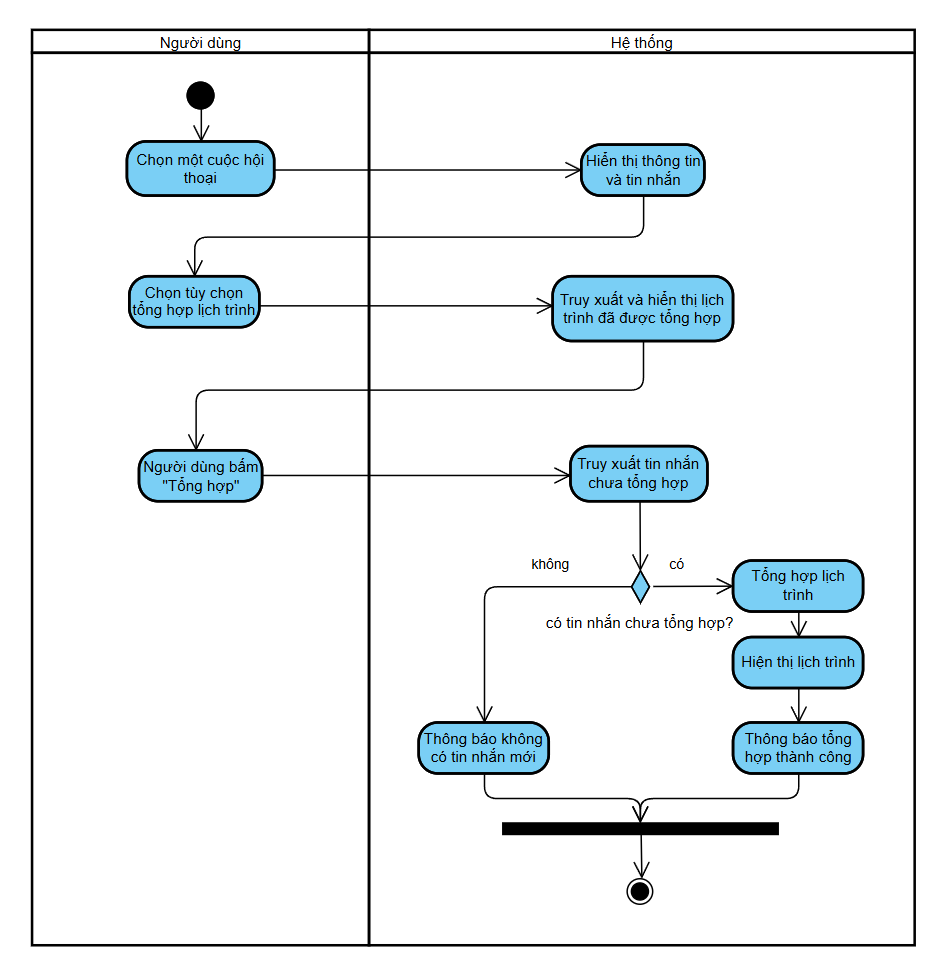
\includegraphics[width=0.5\linewidth]{figures/c3/3-3-10-ad.png} % Specified width
        &
        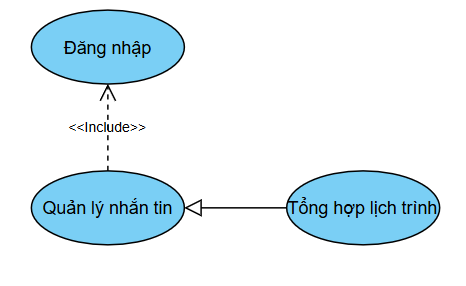
\includegraphics[width=0.45\linewidth]{figures/c3/3-3-10-rd.png} \\ % Specified width
        \hline
    \end{tabular}
\end{table}

\begin{figure}[H]
    \centering
    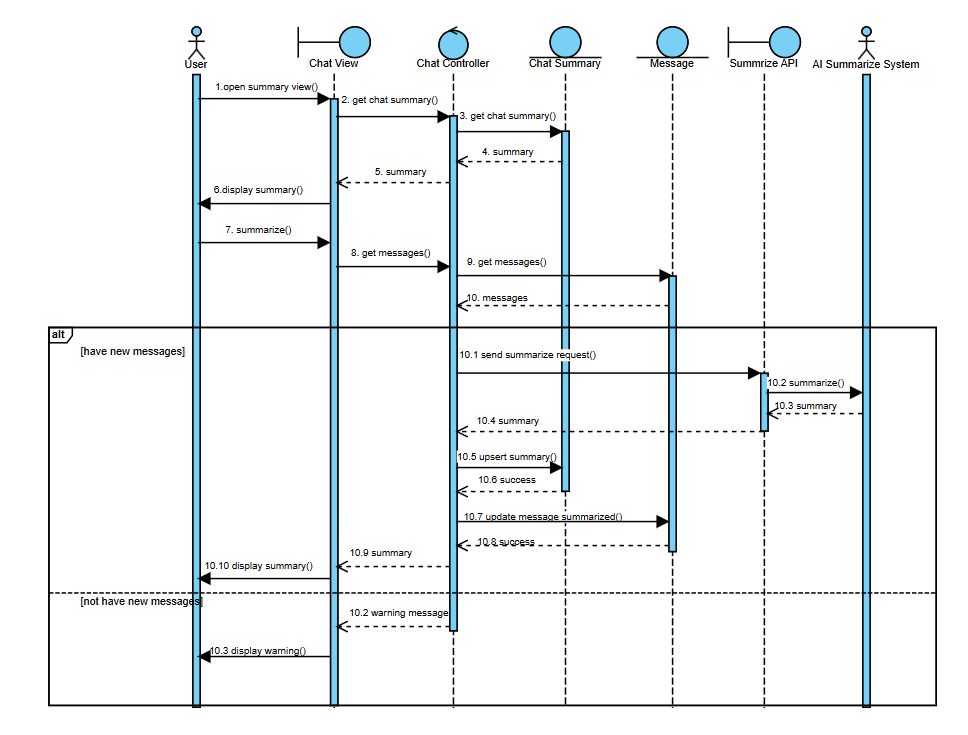
\includegraphics[width=0.95\textwidth]{figures/c3/3-3-10-sd.png} % Specified width
    \caption{Biểu đồ tuần tự ca sử dụng tổng hợp lịch trình từ hội thoại.}
    \label{fig:3-3-10-sequence-diagram}
\end{figure}